\documentclass[aspectratio=169]{beamer}   % 16:9 widescreen

\usetheme{default}
\usecolortheme{default}
\setbeamertemplate{navigation symbols}{}

% ---- minimal, clean look ----
\setbeamercolor{frametitle}{bg=white, fg=black}
\setbeamercolor{background canvas}{bg=white}
\setbeamerfont{frametitle}{size=\Large, series=\bfseries}
\setbeamertemplate{frametitle}[default][center]

\usepackage{amsmath,amssymb}
\usepackage{slashed}
\usepackage{graphicx}
\usepackage{xcolor}
\usepackage{tcolorbox}
\usepackage{tikz}
\usetikzlibrary{arrows.meta, positioning}

\graphicspath{{./figures/}}   % <-- point to the uploaded figures folder

% ---- colours ----
\definecolor{cptblue}{RGB}{0,90,170}
\definecolor{cptred}{RGB}{180,30,30}
\definecolor{cptgreen}{RGB}{20,130,60}
\definecolor{boxbg}{RGB}{230,240,255}


% ============================================================
\begin{document}

% ============================================================
% SLIDE 1 – Title header + Motivation & the two-sheeted structure
% ============================================================
\begin{frame}[t]

  % ---- title header (replaces cover slide) ----
  \begin{columns}[c]
    \begin{column}{0.1\textwidth}
      
\includegraphics[height=1.15cm]{./logos/cambridge-cropped.pdf}
    \end{column}
    \begin{column}{0.9\textwidth}
      \centering
      {\large\bfseries \textit{CPT}-Symmetric K\"{a}hler--Dirac Fermions}\\[2pt]
      {\small Implication in Cosmology \& Fundamental Physics}\\[1pt]
      {\footnotesize Latham Boyle \& Wei-Ning Deng
        |
        Higgs Centre, Edinburgh \& Cavendish/KICC, Cambridge}
    \end{column}
    \begin{column}{0.1\textwidth}
      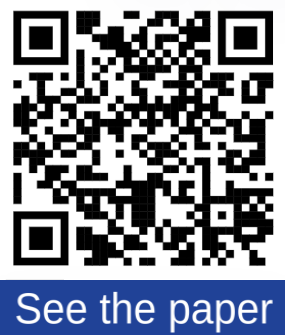
\includegraphics[height=1cm]{./figures/QRcode_arxiv2511.11548}
    \end{column}
  \end{columns}

  \vspace{0.25em}
  {\color{cptblue}\hrule}
  \vspace{0.8em}

  % ---- main content: 3-column narrative ----
  \begin{columns}[T]

    % ---- col 1: CPT universe motivation ----
    \begin{column}{0.31\textwidth}
      \centering
      \textbf{\color{cptblue}CPT-Symmetric Univ.}
      \vspace{0.2em}

      
\includegraphics[width=\linewidth, height=2.5cm, keepaspectratio=false]{figures/CPT_periodic.png}

      \vspace{-0.2em}
      \begin{tcolorbox}[
          colback=boxbg, colframe=cptblue,
          left=3pt, right=3pt, top=2pt, bottom=2pt
        ]
        \footnotesize\centering
        Big Bang $=$ CPT mirror\\
        $\Rightarrow$ solves cosmological const, flatness problem,
        dark matter ($\nu_R$), scale invariant PPS, \textbf{No inflation}
      \end{tcolorbox}

      \vspace{-0.1em}
      \footnotesize\textbf{\color{cptred}%
        But WHY must the Big Bang\\be a CPT mirror?}
    \end{column}

    % ---- col 2: What are KD fermions? ----
    \begin{column}{0.35\textwidth}
      \centering
      \textbf{\color{cptgreen}K\"{a}hler--Dirac Fermions}
      \vspace{0.2em}

      
\includegraphics[width=0.6\linewidth]{lattice.png}

      \vspace{0em}
      \begin{tcolorbox}[
          colback=white, colframe=cptgreen,
          left=3pt, right=3pt, top=2pt, bottom=2pt
        ]
        \footnotesize
        % Spinors have \textbf{no natural lattice definition}
        % $\Rightarrow$ fermion doubling problem.\\[3pt]
        \textbf{KD fermions} are 4D $p$-forms:
          $\Phi = \sum \varphi_{\mu_1\cdots\mu_p}\,
                 dx^{\mu_1}\!\wedge\cdots\wedge dx^{\mu_p}$\\[2pt]
        $(K-m)\Phi= (i\gamma^\mu\partial_\mu - m)\Psi = 0$\\[2pt]
        Live naturally on the lattice
        $\Rightarrow$ \textbf{solve fermion doubling prob.}
      \end{tcolorbox}
    \end{column}

    % ---- col 3: Ghost problem & two-sheet resolution ----
    \begin{column}{0.34\textwidth}
      \centering
      \textbf{\color{cptred}Ghost Problem \& Sol.}
      \vspace{0.2em}

      
\includegraphics[width=0.85\linewidth]{KD_Majorana.png}

      \vspace{0em}
      \begin{tcolorbox}[
          colback=white, colframe=cptred,
          left=3pt, right=3pt, top=2pt, bottom=2pt
        ]
        \footnotesize
        Spinor form $\Psi$ (4$\times$4 matrix):\\
        half the columns have \textbf{wrong-sign} Lagrangian
        $\Rightarrow$ negative-norm states (ghosts)!\\[3pt]
        \textbf{Sol:} wrong sign $=$ $PT$ reversal\\
        $\Rightarrow$ two \textbf{$PT$-symmetric spacetime sheets},
        both with positive energy \& norm.
      \end{tcolorbox}
    \end{column}

  \end{columns}
\end{frame}

% ============================================================
% SLIDE 2 – The KD-Majorana condition & implications
% ============================================================
\begin{frame}
  \frametitle{The KD-Majorana Condition: Field Theory \textit{Forces} CPT}

  \begin{columns}[c]

    % ---- left: equation + SM unification ----
    \begin{column}{0.36\textwidth}

      \begin{tcolorbox}[
          colback=boxbg, colframe=cptblue,
          title={\small\textbf{KD-Majorana condition}},
          fonttitle=\small, left=4pt, right=4pt, top=3pt, bottom=3pt
        ]
          $\Psi^c \equiv (i\gamma^2)\Psi^*(i\gamma^2) = \Psi$
        \small
        Forces every particle on sheet\,1
        to pair with its anti-particle
        on sheet\,2  --- \textbf{CPT is built in.}
      \end{tcolorbox}

      \vspace{0em}

      \begin{tcolorbox}[
          colback=white, colframe=cptgreen,
          title={\small\textbf{SM Unification}},
          fonttitle=\small, left=4pt, right=4pt, top=3pt, bottom=3pt
        ]
        \small
        1 SM generation $= 4$ KD fields\\[1pt]
              $\mathcal{L}_{\rm KD}=
        \mathrm{Tr}\!\left[\bar\Psi_A(i\slashed\partial)\Psi_A\right],$\\$
      \mathcal{L}_Y=
        \mathrm{Tr}\!\left[\mathcal{H}^T
        \widehat\Psi_{A,L}^{\prime\,i}\,\Psi_{A,R}^{\prime\,j}\,
        \mathcal{Y}_A^{ij}\right]$\\[1pt]
        \textbf{$\nu_R$ required by geometry.}
      \end{tcolorbox}

      \vspace{0em}
      \centering
      \footnotesize\texttt{arXiv:2511.11548}

    \end{column}

    % ---- centre: Black Mirror figure ----
    \begin{column}{0.36\textwidth}
      \centering
      \textbf{\color{cptred}Black Mirror}
      {\footnotesize [arXiv:2412.09558]}

      \vspace{0.3em}
      \begin{figure}
        \centering
        
\includegraphics[width=\linewidth]{annihilate_BHmirror.png}
      \end{figure}

      \small
      BH horizon $=$ PT mirror.\\
      Infalling particles \textbf{annihilate}\\
      with anti-partners at the horizon.\\
      {\footnotesize (KD-Maj.\ guarantees every particle has a partner.)}
    \end{column}

    % ---- right: Tenet pop-culture hook ----
    \begin{column}{0.24\textwidth}
      \centering
      \textbf{\color{gray}Sounds like\ldots}

      \vspace{0.3em}
      \begin{figure}
        \centering
        
\includegraphics[width=\linewidth]{tenet_2.jpg}
      \end{figure}

      \vspace{0.2em}
      \footnotesize
      \textcolor{cptgreen}{Same:}\\ T-reversed anti-universe,\\
      BHs as transition gates.\\[3pt]
      \textcolor{cptred}{Different:}\\ you \& anti-you
      \emph{annihilate} at the gate!
    \end{column}

  \end{columns}

  \vfill
  \noindent\begin{tcolorbox}[
      colback=cptblue, colframe=cptblue,
      sharp corners, boxrule=0pt,
      left=6pt, right=6pt, top=3pt, bottom=3pt
    ]
    \color{white}\tiny
    Latham Boyle: \texttt{latham.boyle@ed.ac.uk} \quad\quad
    Wei-Ning Deng: \texttt{wnd22@cam.ac.uk}
    \hfill
    \textbf{arXiv:2511.11548}
    \hfill
    UK Cosmos, London, 2026
  \end{tcolorbox}
\end{frame}

\end{document}
